
%In the following, we first present the performance comparison between original registry and \sysname.
%Next, we present the layer restoring performance.

\subsection{Restore performance of the deduplication cluster}
\label{sec:eval-dedup}

%We map the traces with two different layer groups: 
%small layers (layer size $\leq$ 50 MB)

\begin{figure*}[t]
	\centering
	\begin{minipage}{0.3\textwidth}
		\centering
		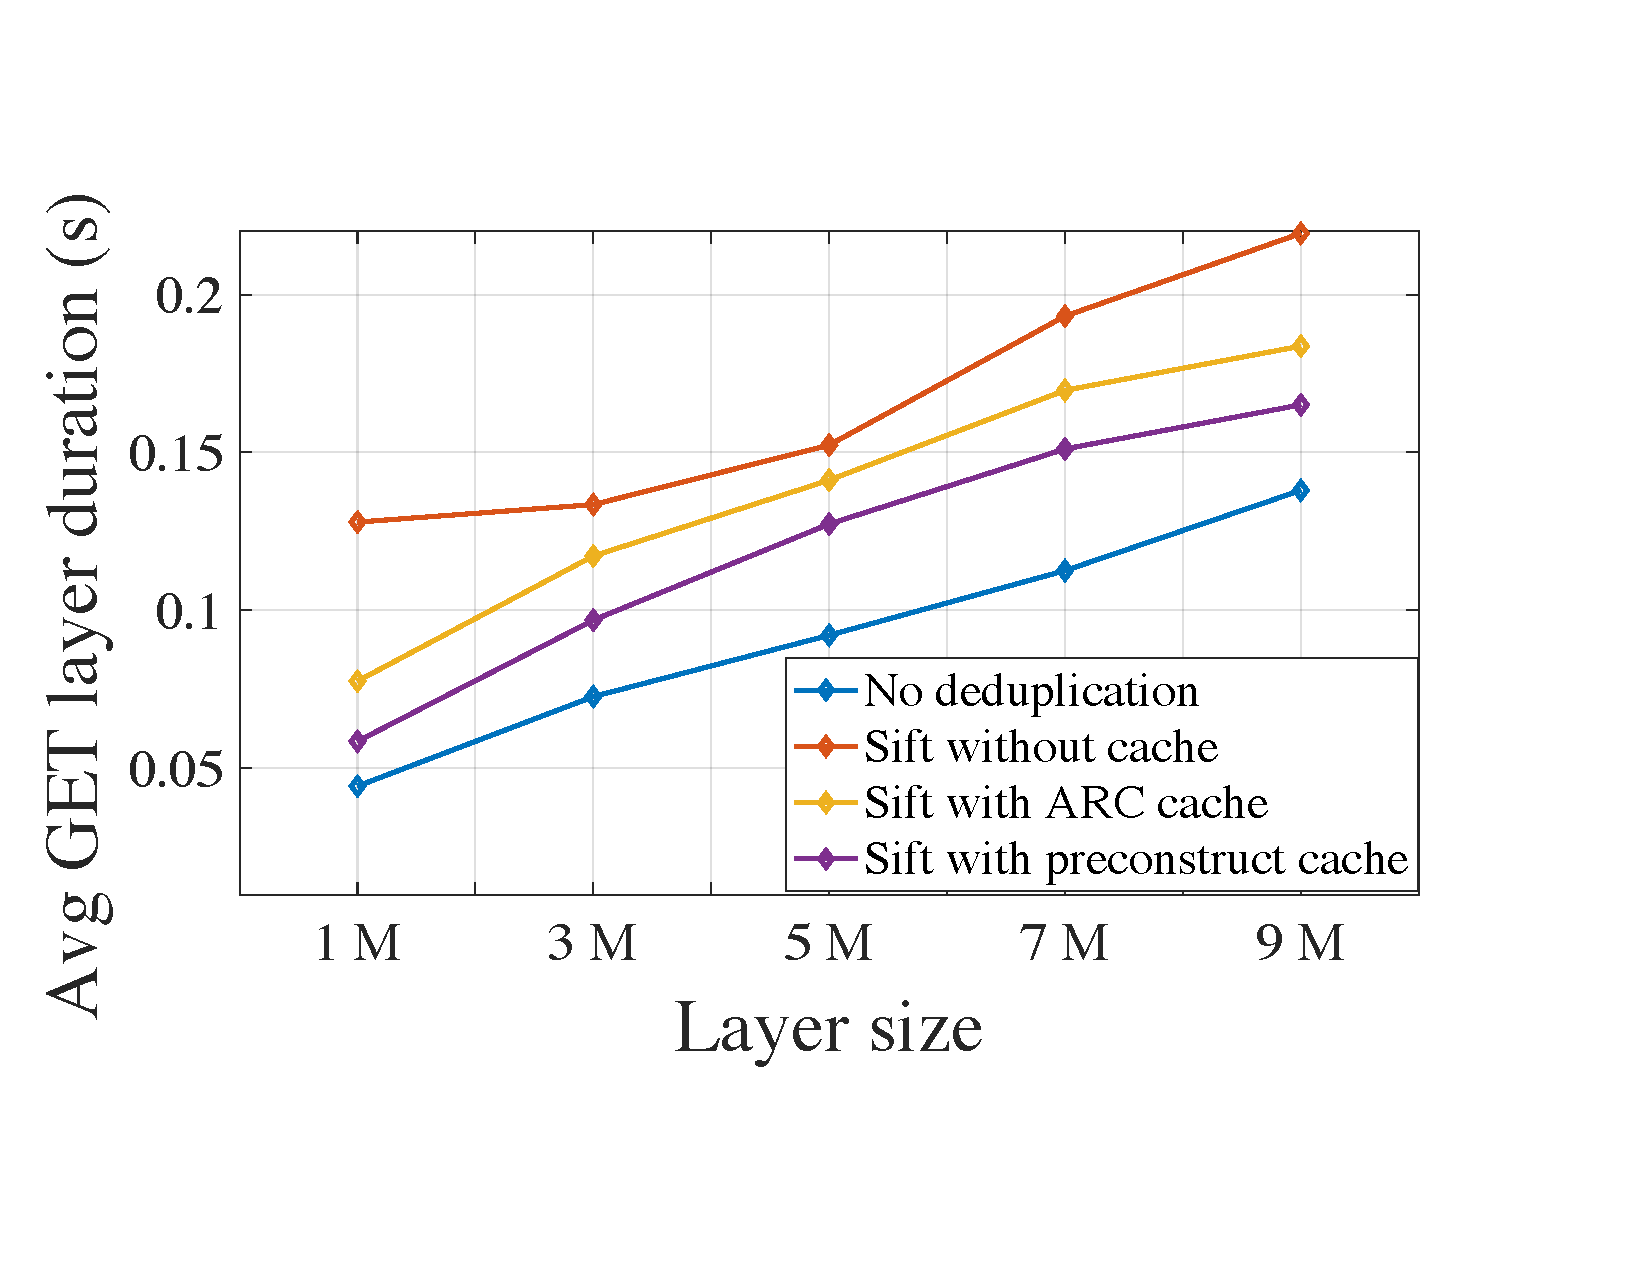
\includegraphics[width=0.9\textwidth]{graphs/1nodegetlayerlatency.pdf}
		\caption{GET layer latency.}% across different schemes.}
		\label{fig:eval-1nodegetlayerlatency}
	\end{minipage}%
	\begin{minipage}{0.3\textwidth}
		\centering
		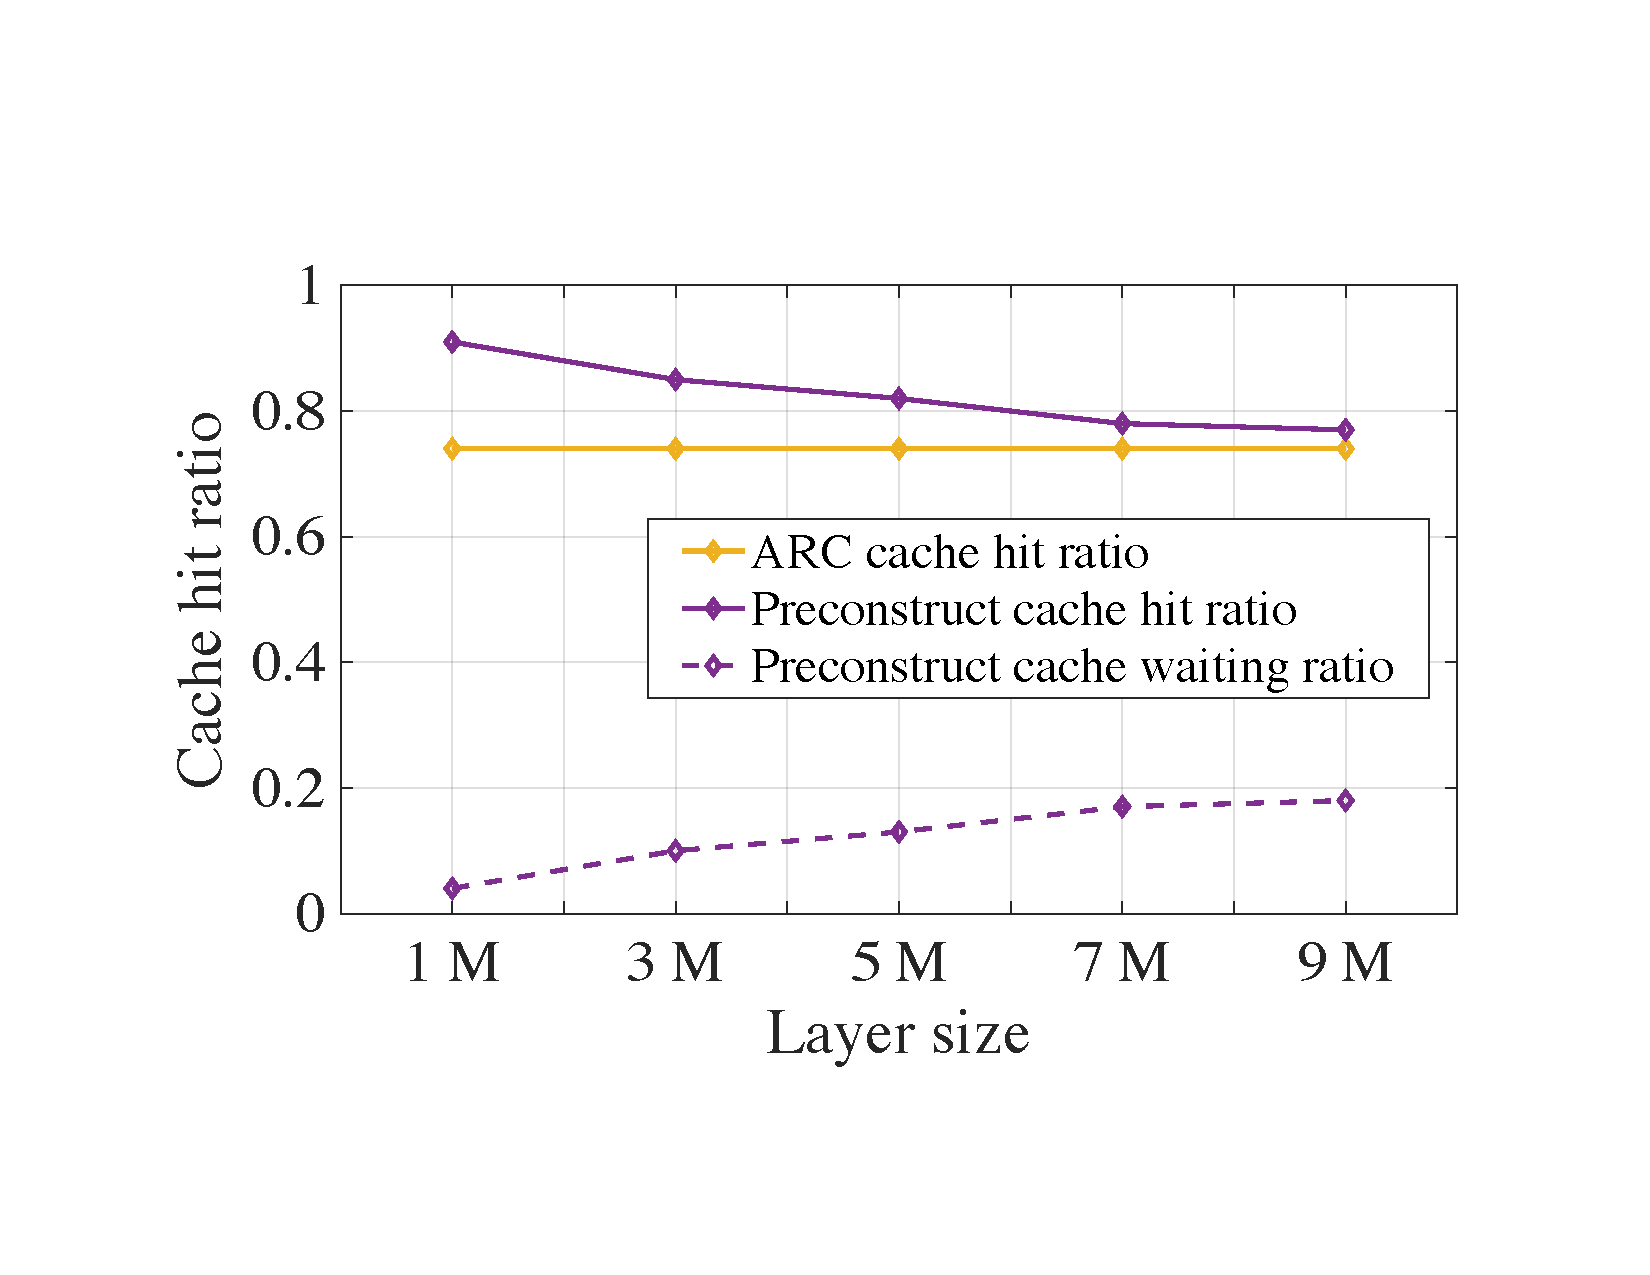
\includegraphics[width=0.9\textwidth]{graphs/cachehitratio.pdf}
		\caption{Cache hit ratio.}% of LRU cache and preconstruct cache.}
		\label{fig:eval-cachehitratios}
	\end{minipage}%
	\begin{minipage}{0.3\textwidth}
	\centering
	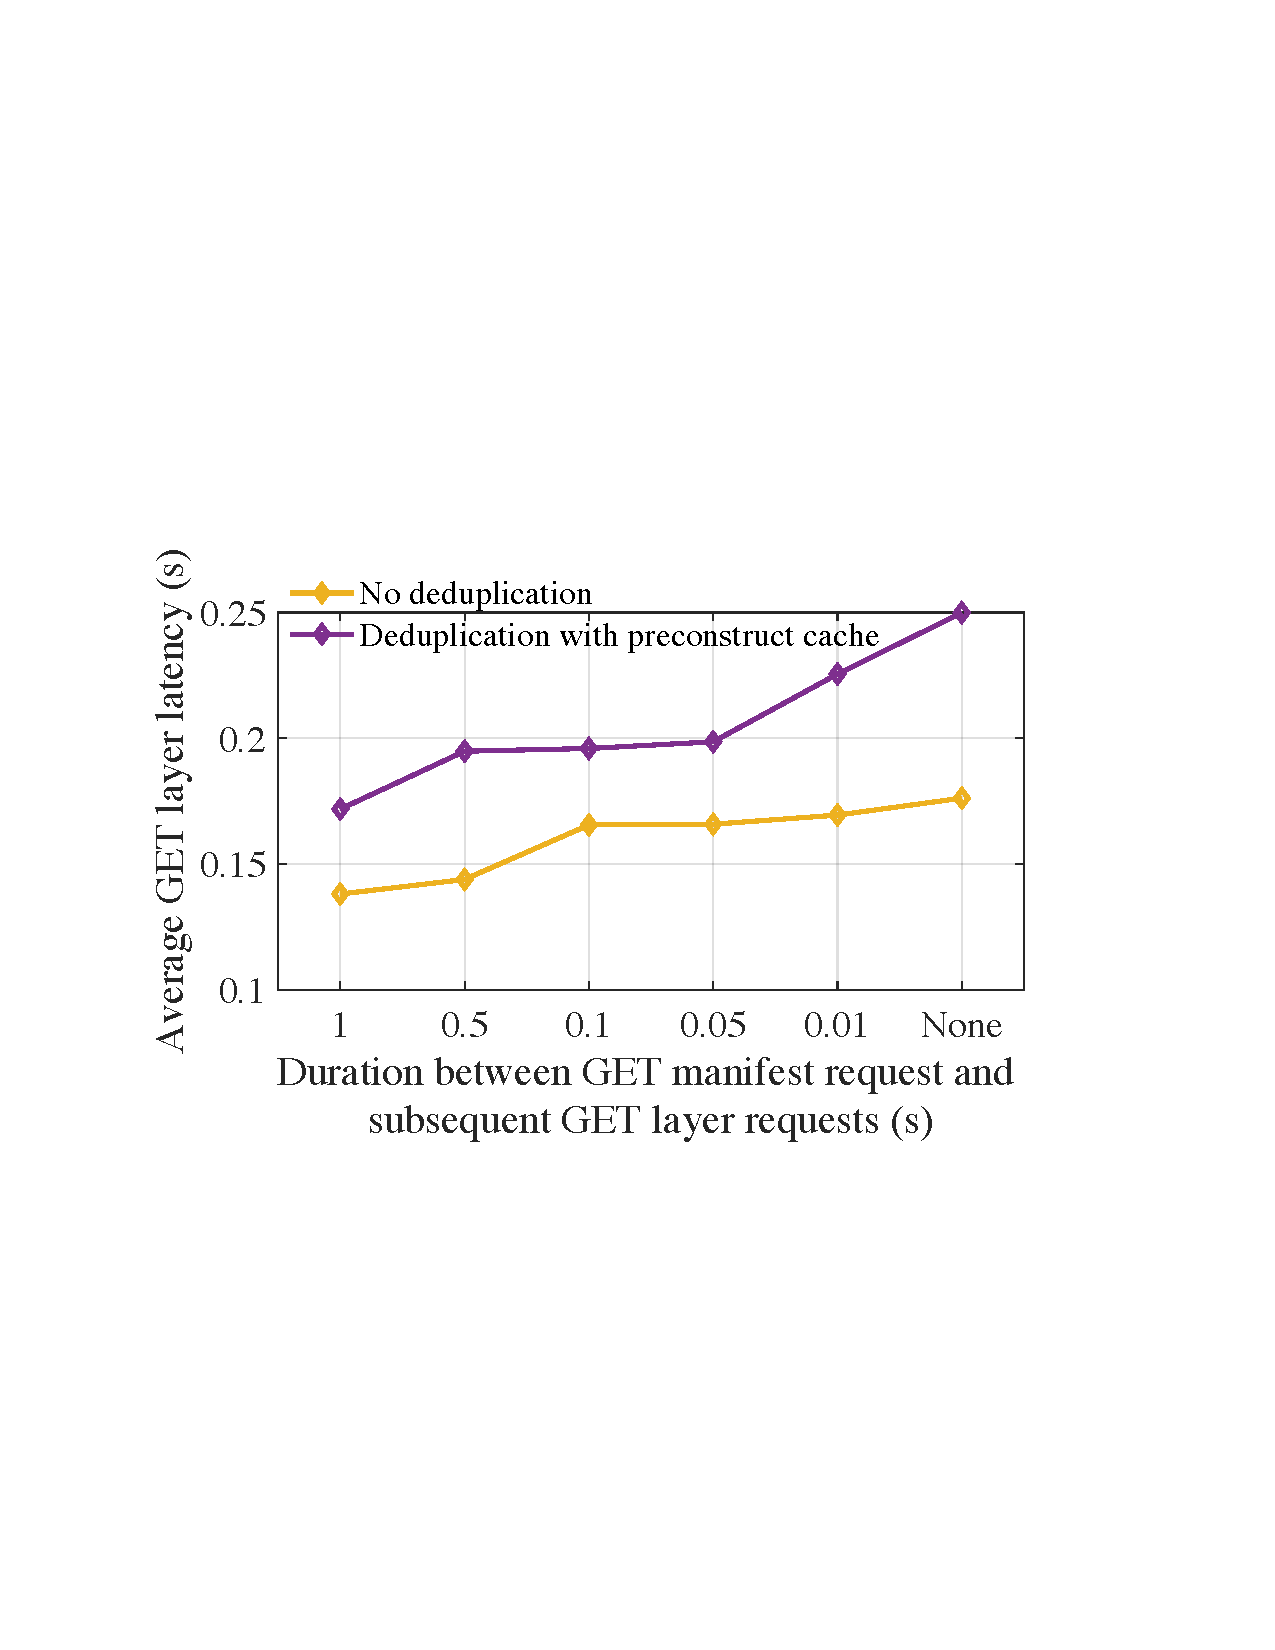
\includegraphics[width=0.9\textwidth]{graphs/durationML.pdf}
	\caption{The impact of durationML.}
	\label{fig:eval-durationML}
   \end{minipage}

\end{figure*}


\begin{figure*}[t]
	\centering
	\begin{minipage}{0.3\textwidth}
		\centering
		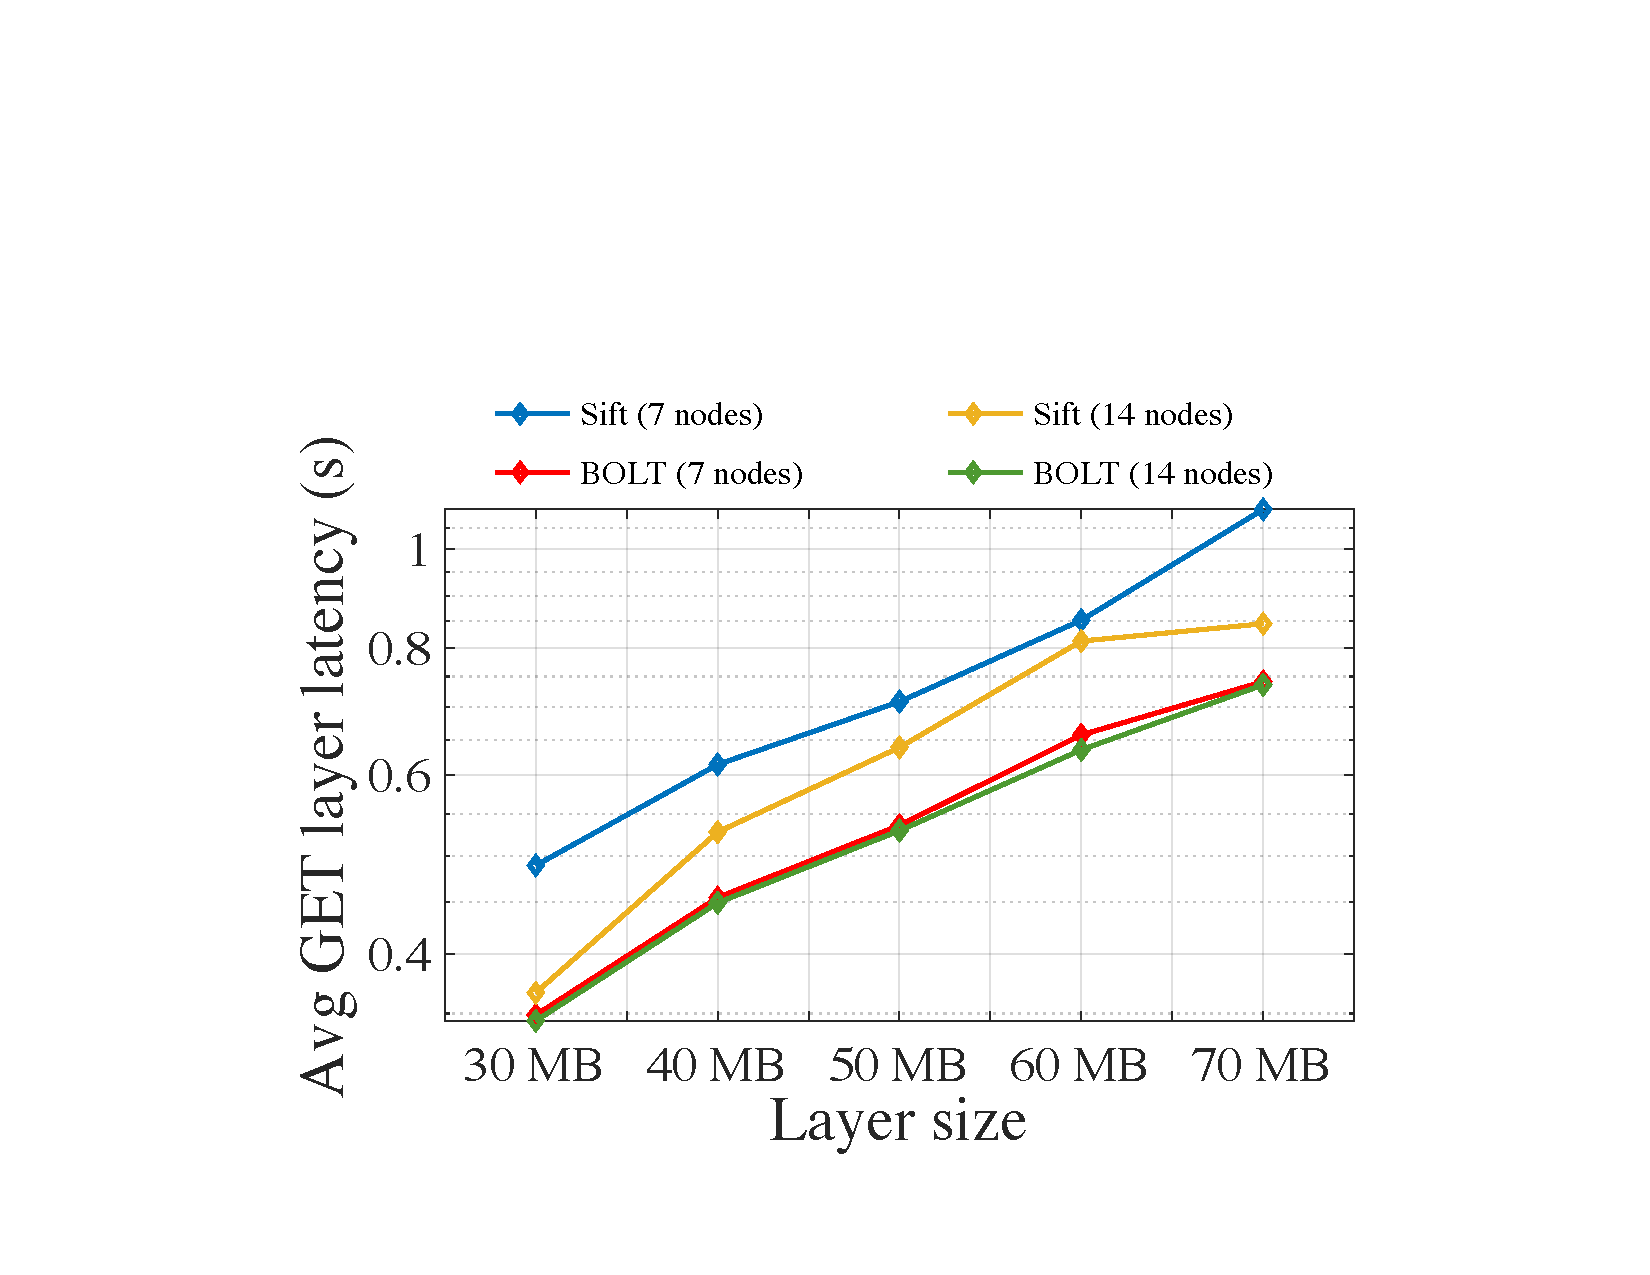
\includegraphics[width=0.9\textwidth]{graphs/clusterscale.pdf}
		\caption{GET layer latency with different cluster size.}
		\label{fig:eval-clusterscale}
	\end{minipage}%
	\begin{minipage}{0.3\textwidth}
	\centering
	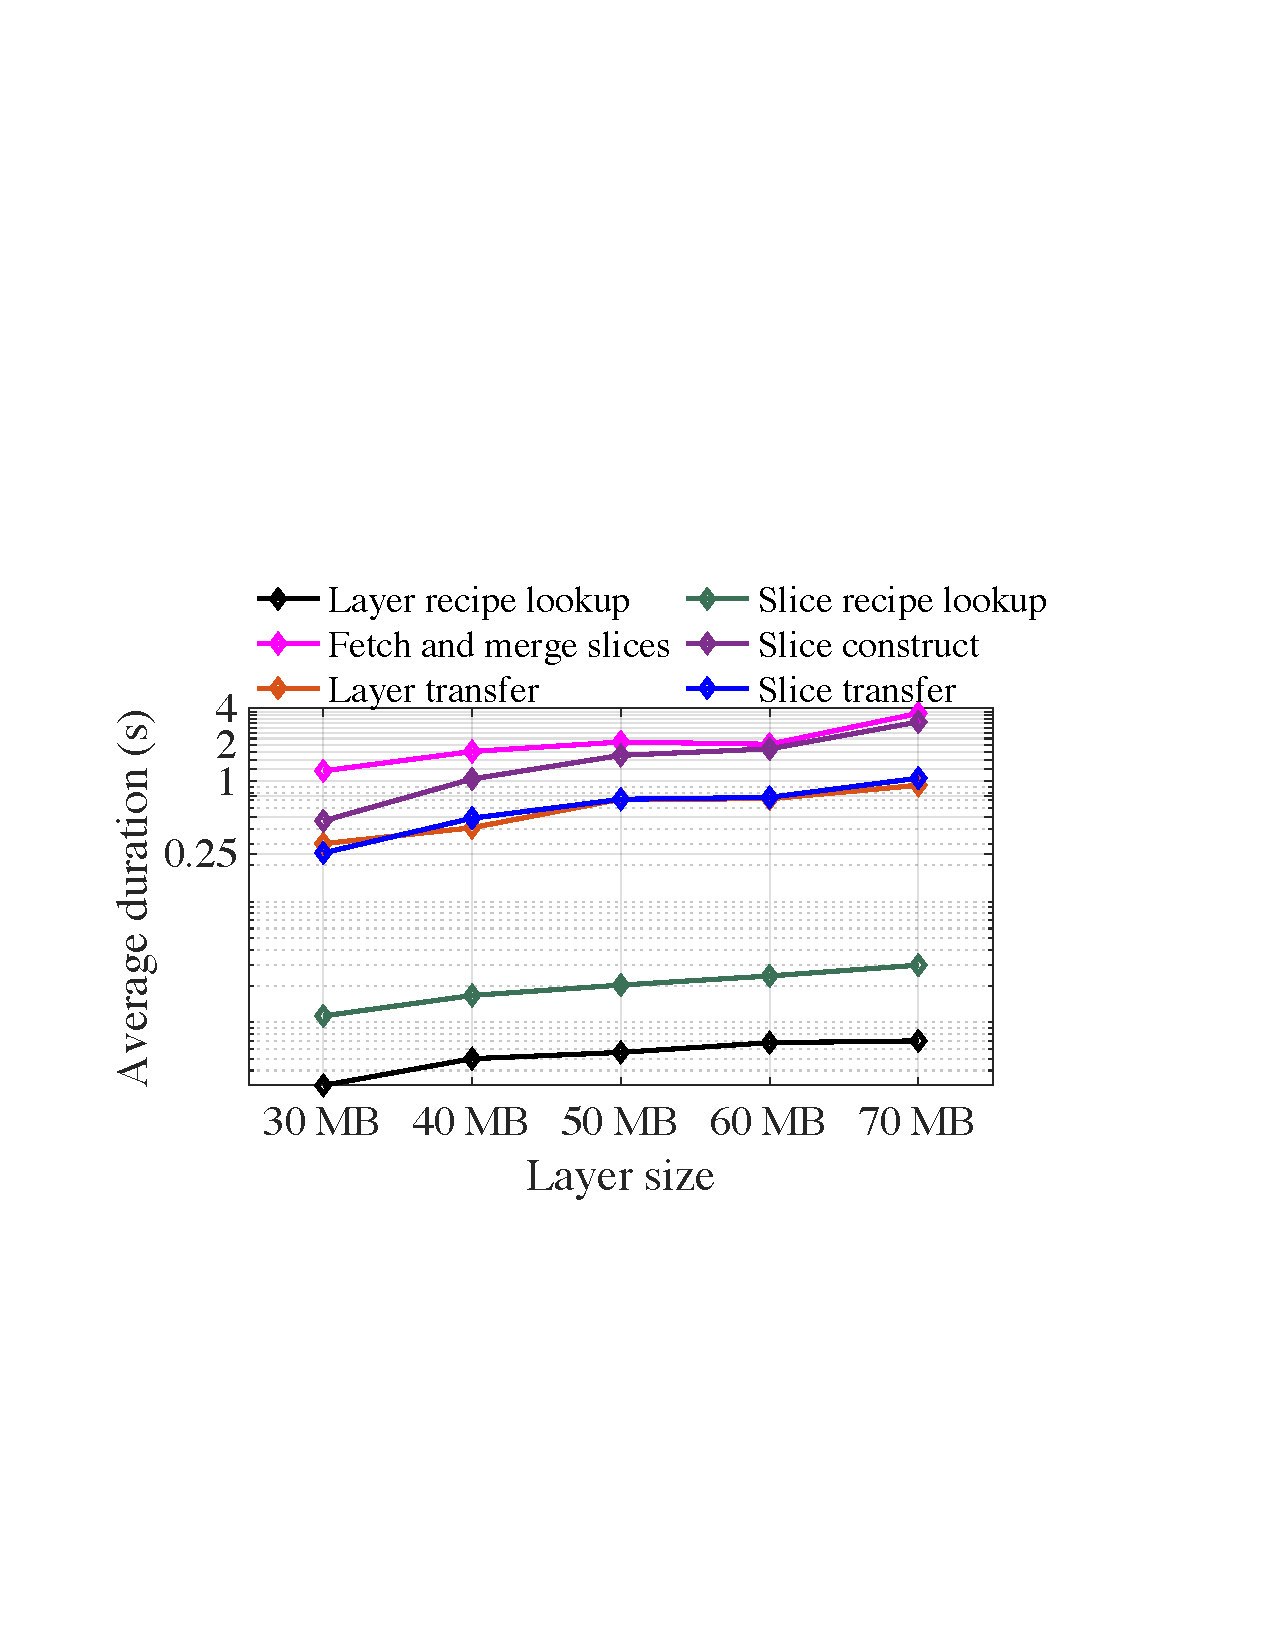
\includegraphics[width=0.9\textwidth]{graphs/restoringbreakdown.pdf}
	\caption{Restoring latency breakdown.}
	\label{fig:eval-restoringbreakdown}
\end{minipage}
	\begin{minipage}{0.3\textwidth}
		\centering
		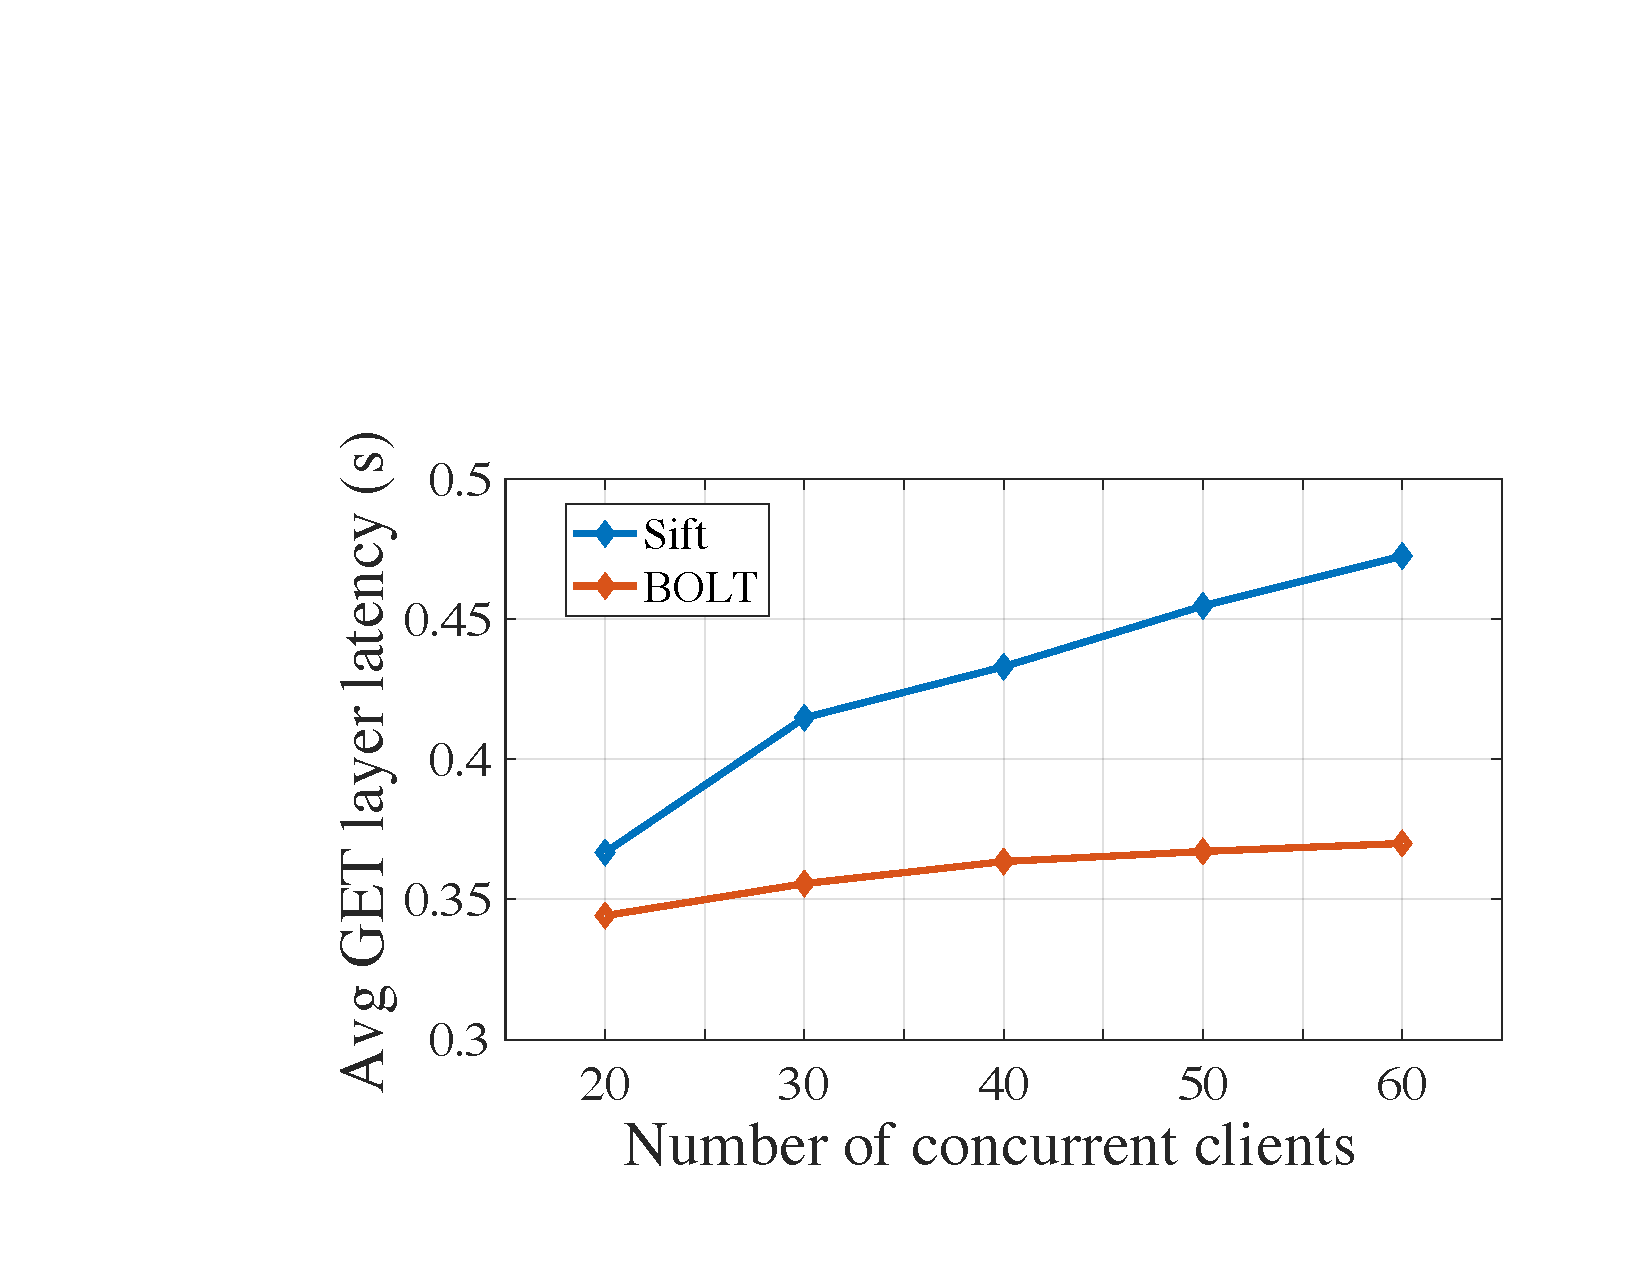
\includegraphics[width=0.9\textwidth]{graphs/clientscale.pdf}
		\caption{GET layer latency with different client concurrency.}
		\label{fig:eval-clientscale}
	\end{minipage}%	
\end{figure*}

\begin{figure}[t]
	\centering
	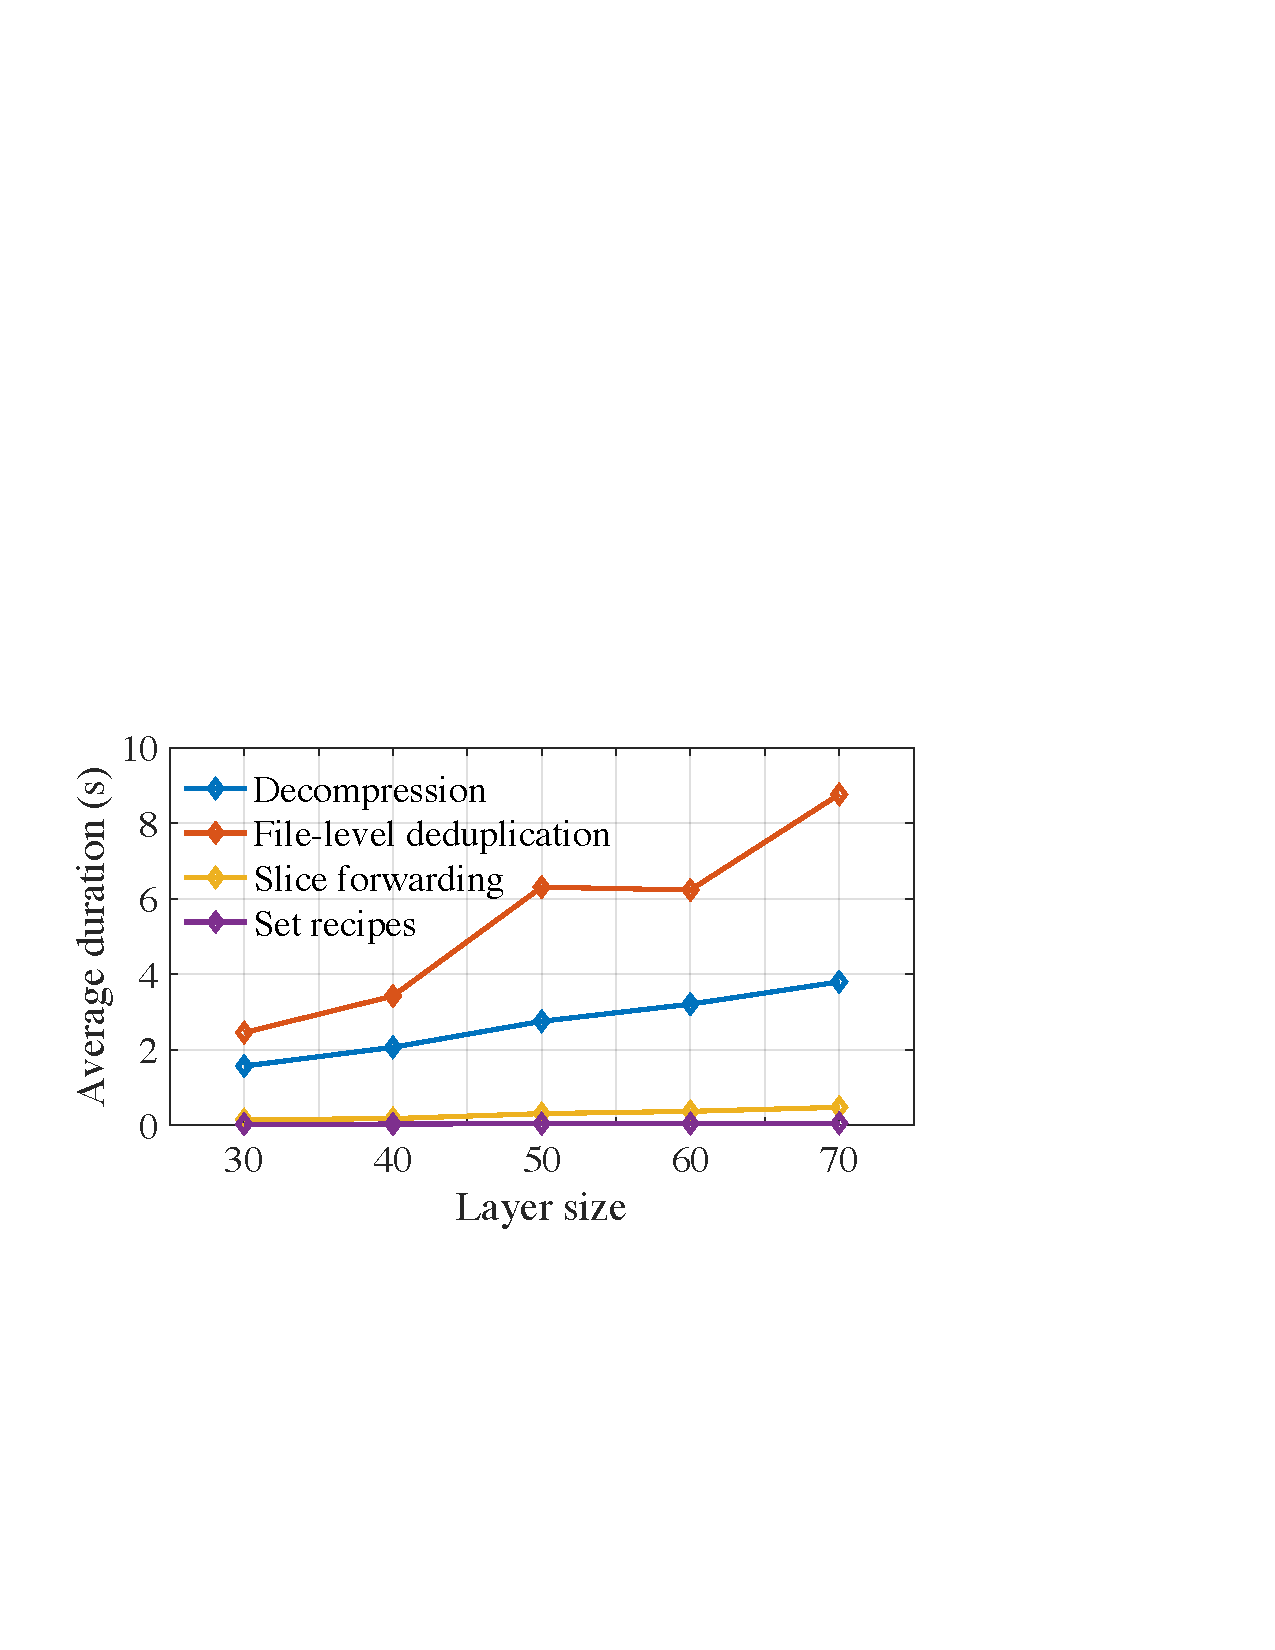
\includegraphics[width=0.3\textwidth]{graphs/dedupbreakdown.pdf}
	\caption{Deduplication latency breakdown.}
	%	\vspace{-3pt}
	\label{fig:eval-dedupbreakdown}
	
\end{figure}

In this experiment, we measure the layer restoring latency of \sysname's deduplication cluster 
and its impact on \texttt{GET} layer request latency.
We first measure a single P-server's layer restoring capability and compare it with 
a \emph{No deduplication} scheme -- 
downloading layers from a plain registry server with local file system as backend
that does no deduplication.
%denoted as .
Then we scale out to a deduplication cluster with multiple P-servers
and compare it with BOLT \cite{littley2019bolt}, 
a consistent hashing based distributed docker registry cluster 
that utilizes the local file systems on the nodes for storage.
%
%
% (denoted as
%\sysname-dedup)
% and 
%overhead of layer deduplication on .
%To measure the  
%We compare the \texttt{GET} layer latency of D-servers
%with 
%by running \sysname with \text{only deduplication} on a single D-server.
%We launch a client on another server and \texttt{pulls} 3 layers in parallel.
%We configure \sysname as
%registry without deduplication,
%deduplication registry,
%deduplication registry with LRU cache~\cite{xxx},
%and
%deduplication registry with a preconstruct cache.
%We set the cache size as 20\% of ingress data.

\paragraph{Restoring latency}
We launch a single node registry on a server and 
a client on another server.
We compare four backends:
(1) Local file system with \emph{no deduplication},
(2) Local file system with \sysname \emph{Deduplication without cache},
(3) Local file system with \sysname \emph{Deduplication with ARC cache}, and
(4) Local file system with \sysname \emph{Deduplication with preconstruct cache}
as shown in Figure~\ref{fig:eval-1nodegetlayerlatency}.
%
The client matches requests from \texttt{Dal} to layers with similar sizes 
from the evaluation dataset and replays them to the D-server.
%We compare four backends: 

As shown in Figure~\ref{fig:eval-1nodegetlayerlatency}, 
layer restoring increases the average \texttt{GET} layer request latency by 189\% for layers 
with size 1~MB in \emph{Deduplication without cache} compared to \emph{No deduplication}.
Moreover, the layer restoring latency increases as the layer size increases.
It takes 0.22~s to restore and download layers with size 9~MB in the \emph{Deduplication without cache} test.

\paragraph{Preconstruct cache VS. ARC cache}
%\paragraph{Cache}
As shown in Figure~\ref{fig:eval-1nodegetlayerlatency}, 
%the average \texttt{GET} layer request latency increase with the layer size.
leveraging a cache can largely reduce layer restoring latency.
By using an ARC cache, 
the layer restoring overhead decreases by 40\% for layers with size of 1~MB compared to \emph{Deduplication without cache}.
However, as the layer size increases, 
the improvement of \texttt{GET} layer request latency due to leveraging ARC cache drops.
For layer sized 9~MB, the ARC cache reduces the layer restoring overhead by only 16\%. 
%\Subil{there is no 10-MB value in Fig~\ref{fig:eval-1nodegetlayerlatency}.}
%ARC cache can only improve 10\% of 
%Restoring a layer puts 150\% overhead on \texttt{GET} layer latency.
%By adding a ARC cache,
%he average \texttt{GET} layer latency decreases by 39\%.
With \sysname preconstruct cache, 
the average \texttt{GET} layer latency for layers 
with size of 1~MB decreases by an extra 24\% over using ARC cache.
%Overall,
Compared to \emph{No deduplication}, 
\sysname with preconstruct cache only adds 19\% of overhead for layers with a 9~MB size. 

\paragraph{Cache hit ratio}
Figure~\ref{fig:eval-cachehitratios} shows the cache hit ratio for ARC cache 
and Preconstruct cache.
Note that the cache size is set to 20\% of \texttt{Dal}'s ingress data.
%\Subil{approximately how much is Dal's ingress data?}.
The cache hit ratio for ARC is stable at 0.77 for all layer sizes.
%However, 
Preconstruct cache achieves a hit ratio of 0.95 for 1 MB.
As the layer size increases to 9~MB, the preconstruct cache hit ratio decreases to 79\%. 
This is because the layer restoring latency increases with layer size as shown in Figure~\ref{fig:eval-1nodegetlayerlatency} and therefore, 
many layers are not preconstructed on time.
% and more layers cannot be preconstructed \emph{on time} as the layer size increases. 
As shown in Figure~\ref{fig:eval-cachehitratios}, 
the number of waiting \texttt{GET} layer requests increases with layer size, depicted by the preconstruct cache waiting ratio.
Since layer construction already starts before these requests arrive, the restoring overhead can be reduced.
The user-bahavior based request prediction accuracy is calculated by summing the preconstruct cache hit ratio and the waiting ratio.
As shown in Figure~\ref{fig:eval-cachehitratios}, the prediction accuracy is 0.95.
 
\paragraph{Impact of duration between a \texttt{GET} manifest request and its subsequent \texttt{GET} layer requests}
Next, we vary the duration between a \texttt{GET} manifest request and its subsequent \texttt{GET} layer requests (denoted as \emph{durationML}).
The layer size used here is 9~MB.
%
Figure~\ref{fig:eval-durationML} shows the average \texttt{GET} layer latency for \sysname deduplication with preconstruct cache versus \emph{No deduplication}.
When the durationML is 1~s, \sysname with preconstruct cache only imposes a 19\% overhead.
However, as the durationML decreases, the average \texttt{GET} layer latency increases because layers are not preconstructed on time.
When the client replays requests as fast as possible, the overhead of restoring layers on \texttt{GET} layer requests increases by 30\%.

%the cache hit ratio of the ARC cache and the preconstruct cache.

\paragraph{Cluster scale impact}
We scale the backend storage system to show how the \texttt{GET} layer performance changes. 
 %To do that,
 %we launch multiple registries on each registry server. 
The backends are:
 (1) \sysname deduplication cluster (denoted as \sysname-dedup),
 and
 (2) BOLT \cite{littley2019bolt}.
 We implement layer deduplication on the
 local file system of each registry server.
We implement consistent hashing logic on the client side (see \S\ref{sec:impl}) to distribute requests across the cluster of our deduplication registry servers.
 %Besides, 
 %that the client distributes layers to 
%Therefore,
%we also use our client to cluster the non-dededuplication registry servers and setup BOLT for evaluation.
We increase the number of registry servers from 7 to 14,
and the layer sizes from 30 to 70.
We launch 20 clients to replay requests to the registries.
%
%\sysname deduplication cluster and test the layer restoring performance.
As shown in Figure~\ref{fig:eval-clusterscale}, 
when the number of servers increases, 
the average \texttt{GET} layer latency for BOLT doesn't changes much.
However, the performance of \sysname scales with the number of servers.
This is because with a bigger deduplication cluster, the layer restoring latency is largely reduced as layer restoring has a higher parallelism level. 
As shown in Figure~\ref{fig:eval-clusterscale}, when the layer size is 30~MB, doubling the cluster size reduces 35\% of the restoring overhead.

\paragraph{Restoring latency breakdown}

Figure~\ref{fig:eval-restoringbreakdown} shows 
the layer restoring latency breakdown.
The layer restoring latency comprises layer recipe lookup duration, layer construction duration, and layer transfer duration.
The layer construction duration involves slice recipe lookup duration, slice construction, and slice transfer duration.
%
The latencies are measured on the 7-node cluster.
The layer restoring latencies shown in Figure~\ref{fig:eval-restoringbreakdown} only include complete layer restoring processes. 
We eliminate the layer restoring processes that are waiting for others to construct layers.
Note that the layer restoring latencies measured also include layer restoring processes for preconstruction.

As shown in Figure~\ref{fig:eval-restoringbreakdown}, slice construction duration accounts for the largest portion of layer construction time.
Slice construction involves file archiving and compression, which are two bottlenecks of slice construction. 
Layer construction time increases with layer size because layer slices become bigger and take a longer time to archive and compress.
For example, for layers of size 30~MB, fetching and merging slices take 1.3~s on average.
When the layer size increases to 70~MB, it takes 3.6~s on average to fetch and merge slices.

\paragraph{Client concurrency impact}
We increase the number of concurrent client requests and measure the average \texttt{GET} layer request latency on a 14-node cluster for \emph{\sysname-dedup} and a \emph{BOLT}.
%
Figure~\ref{fig:eval-clientscale} shows
the average \texttt{GET} layer latency for \emph{\sysname-dedup} and \emph{BOLT} for a varying number of concurrent client requests.
The \texttt{GET} layer latency for BOLT is almost stable as the number of clients increase.
However, for \emph{sift-dedup}, the average \texttt{GET} layer request latency increases with the number of concurrent client requests.
For example, in the case of \emph{\sysname-dedup}, when the number of concurrent client requests is 20, the average \texttt{GET} layer request latency is 0.37~s while when it's 60, the average \texttt{GET} layer request latency  increases to 0.47~s.
This is because layer restoring process is computationally intensive.
The more concurrent requests, the higher the layer restoring overhead.

\paragraph{Deduplication latency breakdown}
Figure~\ref{fig:eval-dedupbreakdown} shows the breakdown of the deduplication latency.
Note that to reduce the impact of layer deduplication on the \texttt{GET} layer request, the layer deduplication process is single-threaded and off-line \Subil{This conflicts with our description of pgzip in the Implementation section where we talk about using parallelism in both compression ad decompression}.
As shown in Figure~\ref{fig:eval-dedupbreakdown}, decompression and file-level deduplication account for the largest portions of the layer deduplication duration.
This is because \sysname uses single-threaded decompression and file-level deduplication for reducing the computation overhead of the off-line layer deduplication.
Moreover, the duration of decompression and file-level deduplication increases with layer sizes.
For example, when the layer size increases from 30~MB to 70~MB, 
the decompression duration increases from 1.6~s to 3.8~s on average and the file-level deduplication duration increases from 2.5~s to 8.8~s on average.
%\paragraph{Metadata size} 
%Figure~\ref{xxx} shows the average metadata size on each registry server measured by using the size of the used memory in Redis~\cite{redis} when in \emph{B-mode 0}.
%Note that the replication level for the Redis cluster is also set to three.
%As shown, for all traces, the total size of the metadata generated by \sysname such as \emph{recipes} for layers or slices, \emph{indexes} of layers or files, and RLmap or ULmap is less than 100 MB.
%With the 16 GB memory on each registry server, such metadata size is negligible.


